\section{Success Rate and Guessing Entropy}

% intro to SR and GE
\begin{frame}
    \frametitle{Success Rate (SR) and Guessing Entropy (GE): Introduction}
    
    \begin{block}{Motivation}
        \begin{itemize}
            \item In known-key analysis, \textbf{evaluators} have access to the secret key. This allows for more precise security assessments.
            \item SR and GE metrics move beyond a simple "key recovered/not recovered" statement to quantify the attack's probabilistic progress.
        \end{itemize}
    \end{block}
    
    \begin{block}{What is Success Rate (SR)?}
        \begin{itemize}
            \item \textbf{SR} measures the probability that an attack successfully places the correct key candidate at \textbf{rank 1}.
            \item It is derived from the attack's guess vector: if the top guess (\texttt{guess\textsubscript{1}}) matches the correct key, the experiment is a success.
            \item To ensure statistical stability, SR is typically computed by averaging results over many repeated attack experiments.
        \end{itemize}
    \end{block}
\end{frame}

% Slide 2: Success Rate (SR): Definition
\begin{frame}
    \frametitle{Success Rate (SR): Definition}
    
        Recall that a standard side-channel attack produces a guess vector $[guess_1, guess_2, \dots, guess_{|K|}]$ where $guess_1$ is the best candidate. \newline
        Let $k_c$ be the correct key.    
    \begin{block}{Formal Definition}
        For a side-channel experiment $i$, the success rate $SR_i$ is 1 if the best guess equals the correct key ($guess_1 = k_c$), otherwise it's 0.
        Alternatively, using the rank of the correct key (rank $k_c$):
        $$ SR_i = \begin{cases} 1, & \text{if } rank_{k_c} = 1 \\ 0, & \text{otherwise} \end{cases} $$
        To ensure statistical stability, the final SR metric is estimated by averaging over $p$ experiments:
        $$ SR = \frac{1}{p} \sum_{i=1}^{p} SR_i $$
    \end{block}
\end{frame}

% Slide 3: Success Rate (SR): Interpretation and Order
\begin{frame}
    \frametitle{Success Rate (SR): Interpretation}
    Increasing the number of attack traces typically improves the success rate gradually.
    An $SR$ value closer to 1 implies a high probability of correct key recovery. \newline % Add vertical space

    Full key recovery implies $SR=1$. However, we often want the SR metric to reflect cases where the correct key is ranked highly, yet $>$ 1. 
    \newline

    \begin{figure}[htbp]
        \centering
        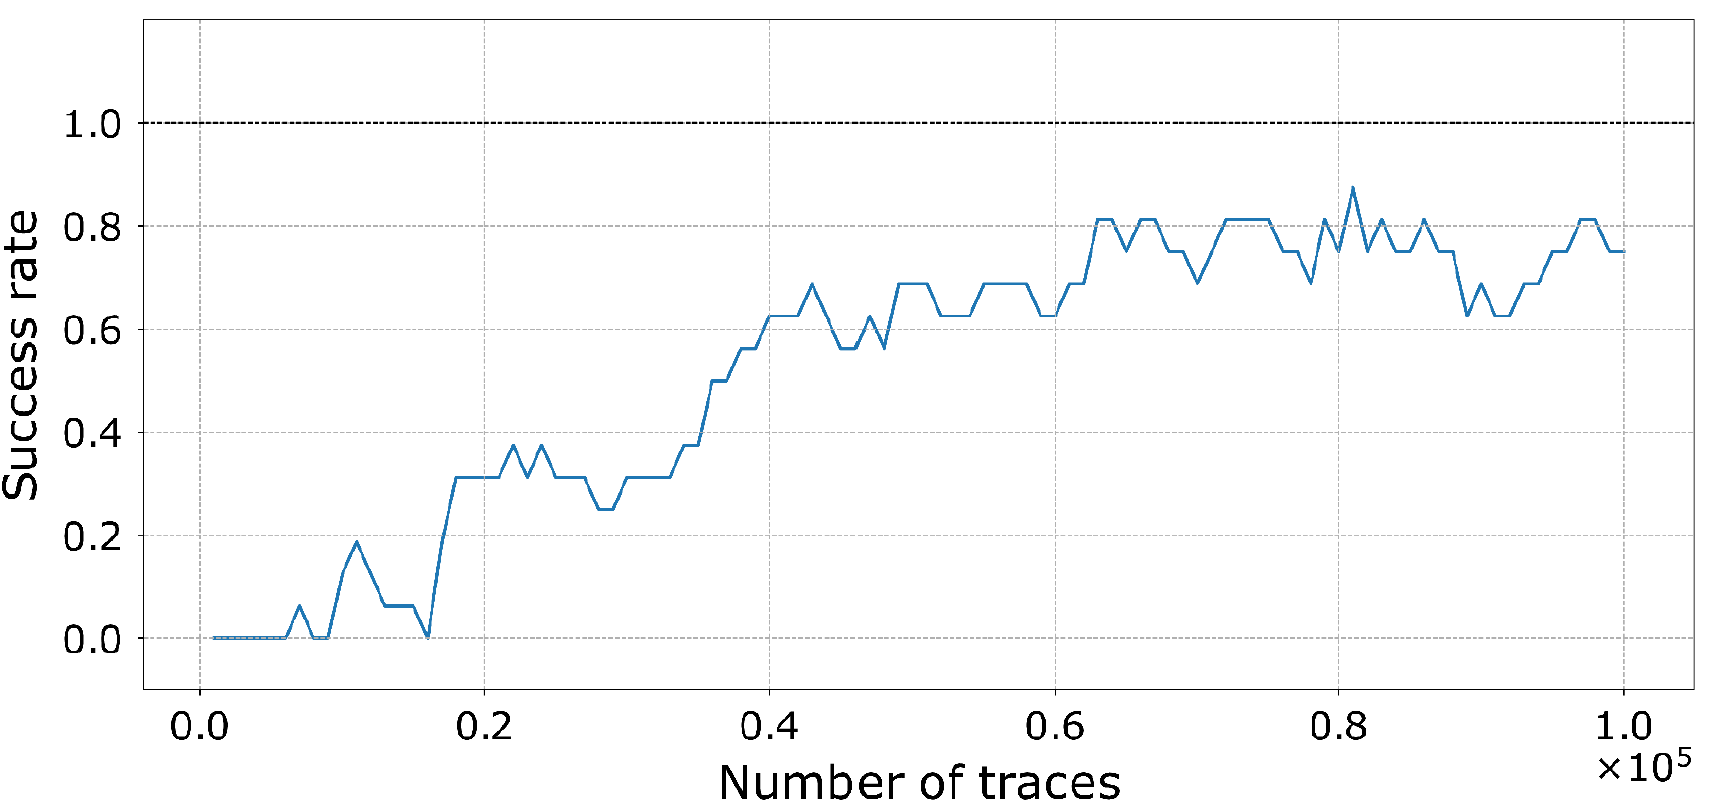
\includegraphics[width=0.8\textwidth]{metrics/Pictures/SR_plot_unprotected.png}
        \caption{for an unprotected AES using 16 parallel S-boxes, $SR$ (with 100,000 traces) is 1 only 80\% of the time}
    \end{figure}
\end{frame}
\begin{frame}
    \begin{block}{SR of Order $o$}
        The $SR$ metric can be extended to reflect cases where the correct key is ranked highly, but not necessarily 1st.
        
        $SR_i^o$ is 1 if the correct key $k_c$ is found within the top $o$ key guesses (i.e., $k_c \in [guess_1, \dots, guess_o]$ or $rank_{k_c} \le o$), otherwise 0.
        $$ SR_o^i = \begin{cases} 1, & \text{if } rank_{k_c} \le o \\ 0, & \text{otherwise} \end{cases} $$
        The overall $SR_o$ is:
        $$ SR_o = \frac{1}{p} \sum_{i=1}^{p} SR_o^i $$
        If $o=1$, this reverts to the original $SR$ definition.
    \end{block}
\end{frame}


% Slide 4: SR of Order 'o' and Attacker Effort
\begin{frame}
    \frametitle{SR of Order $o$: Link to Attacker Effort}
        If an evaluator finds $SR^o=1$ for a key part, an attacker with an unknown key would need to verify at most $o$ candidates to find that key part after performing the attack.
        \newline
        \textit{Example:} If $SR^5=1$ for an AES byte, the attacker needs to check at most 5 candidates for that byte.
    
    \begin{block}{Full Key Enumeration Challenge}
        \begin{itemize}
            \item This key enumeration process must be repeated for all divide-and-conquer partitions of the full key.
            \item For example, if $SR^5=1$ for all 16 AES-128 key bytes, an attacker might need to verify up to $5^{16}$ full keys.
            \item This is a computationally challenging, heuristic task, and determining the appropriate value for $o$ is critical for assessing attacker capability.
        \end{itemize}
    \end{block}
\end{frame}

% Slide 5: Guessing Entropy (GE): Definition
\begin{frame}
   
    \frametitle{Guessing Entropy (GE): Definition}
    
        To avoid the heuristic and potentially complex process of $SR$ of order $o$ for full key enumeration, Guessing Entropy (GE) offers a more flexible metric.
   
    
    \begin{block}{GE Formal Definition}
        Given a rank vector $[rank_0, rank_1, \dots, rank_{|K|-1}]$ and the correct key $k_c$, the rank of $k_c$ ($rank_{k_c}$) can be found and plotted against the number of traces.
        
        For a given experiment $i$, $GE_i$ is defined as:
        $$ GE_i = \log_2(rank_{k_c}) $$
        It is typically expressed in bits.
        
        The overall GE, averaged over $p$ experiments (where $k_c$ is ideally changed between experiments to ensure statistical stability), is:
        $$ GE = \frac{1}{p} \sum_{i=1}^{p} GE_i $$
    \end{block}
\end{frame}



\begin{frame}
    \frametitle{Guessing Entropy (GE): Interpretation and Example}

        The $rank_{k_c}$ and GE metrics represent the average remaining workload for an attacker after a side-channel attack.
        GE = 0 means the side-channel attack has eliminated all uncertainty about the secret key
            %\item For masked S-box implementations, GE stays substantially above 0 (about 8 bits even with 50,000 traces), showing that the attack leaves significant uncertainty and the device remains resistant.

    \begin{figure}
        \centering
        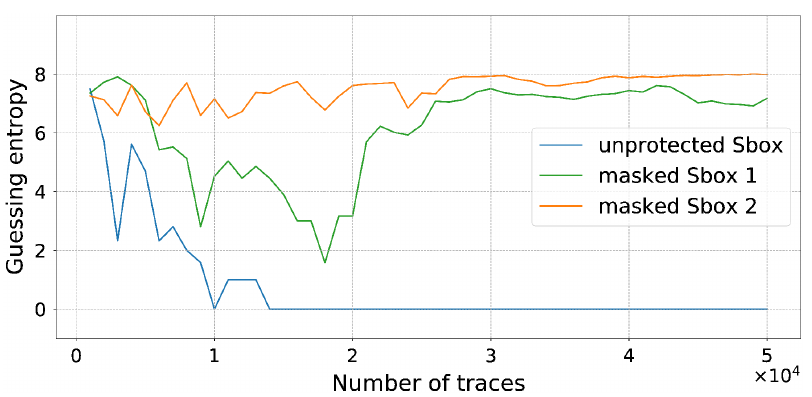
\includegraphics[width=0.75\textwidth]{metrics/Pictures/GE_plot.png}
        \caption{Guessing Entropy plot for three AES S-box implementations. GE drops to 0 for the unprotected S-box after roughly 15,000 traces; for masked S-boxes, GE remains high even with 50,000 traces.}
    \end{figure}
\end{frame}

%%%%REVIEW
\begin{frame}
    \frametitle{Limitations of SR and GE: Full Key Security}

    \begin{block}{Byte-wise Metrics Do Not Translate Directly}
        Both Success Rate (SR) and Guessing Entropy (GE) quantify attack effectiveness for individual key bytes (e.g., in AES). However, knowing the GE or SR for all bytes does \textbf{not} allow direct inference of the GE or SR for the full key.
    \end{block}

    \begin{itemize}
        \item The process of full key recovery requires \textbf{key rank estimation}, which is the known-key analog of key enumeration.
        \item Full key security assessment is more complex than simply combining values for each byte; detailed estimation methods are required.
    \end{itemize}
\end{frame}

\begin{frame}
    \frametitle{Limitations of SR and GE: No Projection of Effort}

    \begin{block}{Trace-Dependency Limits Security Forecast}
        SR and GE provide attack progress for a specific number of measured traces, but do not project future effort required for successful key recovery.
    \end{block}

    \begin{itemize}
        \item If SR or GE is close to random guessing (e.g., 1/256 for AES byte), one can only conclude the attack currently fails.
        \item The metrics do \textbf{not} indicate how many more traces would be needed to break the cipher, nor are they designed to forecast eventual success.
        \item GE is an expression of the remaining effort, but it is always derived from a specific number of measured traces.
    \end{itemize}

    \begin{block}{Towards Better Projections}
        This limitation led to the development of new metrics, which tie attack scores and success probabilities more rigorously to the number of traces.
    \end{block}
\end{frame}

